\documentclass[12pt,a4paper]{exam}

% --------------------
% Packages
% --------------------
\usepackage[utf8]{inputenc}
\usepackage[T1]{fontenc}
\usepackage[french]{babel}
\usepackage{amsmath,amssymb}
\usepackage{geometry}
\usepackage{pgfplots}

\pgfplotsset{compat=1.18}
\geometry{margin=2cm}

% --------------------
% En-tête / pied (exam)
% --------------------
\header{\textbf{NOM Prénom :} }{}{4\up{ème} 1}
\footer{}{\thepage}{\it{G.M.}}

% --------------------
\begin{document}

\begin{center}
    \Large\textbf{Contrôle de mathématiques\\Thalès et calcul littéral}
\end{center}

\vspace{0.3cm}

\noindent
\textbf{Durée :} 1h \hfill
\textbf{Calculatrice :} \underline{autorisée} 

\vspace{0.5cm}

% ======================================================
\noindent
\textbf{\large{Exercice 1 : Hauteur d'un immeuble} (\ \ \ \  / 8 points )}
\vspace{5pt}

Lucie souhaite connaître la hauteur de son immeuble. À 45 mètres de celui-ci se trouve 
un arbre de 8 mètres de haut. Elle recule de 5 mètres depuis l'arbre afin que son regard 
soit aligné avec la cime de l'arbre et le haut de l'immeuble.

\vspace{5pt}
Dans la figure ci-dessous, 
qui n'est pas à l'échelle, on a symbolisé la façade de l'immeuble par le segment $[IM]$, 
l'arbre par le segment $[AR]$ et le regard de Lucie par le point $L$. On estime que le regard 
de Lucie se trouve à 1,60m du sol.

\begin{center}
    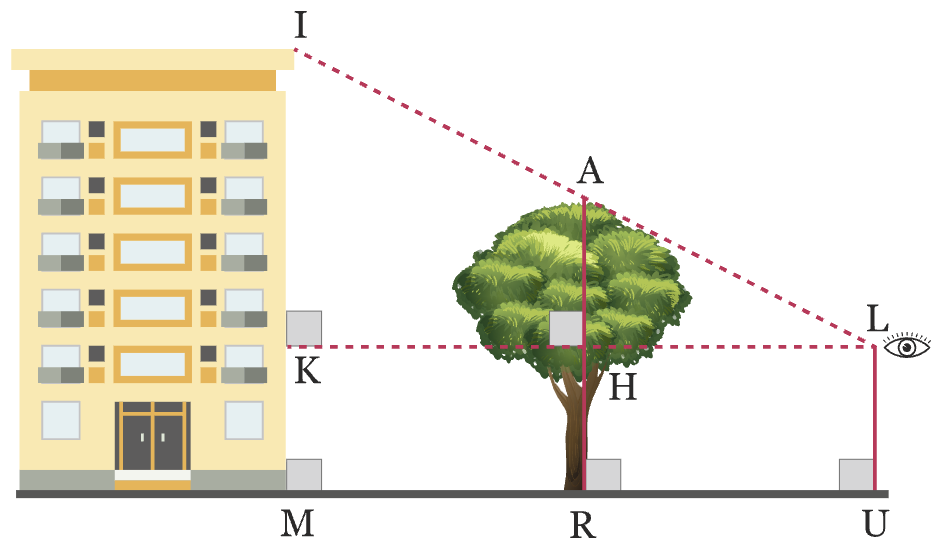
\includegraphics[width=0.7\textwidth]{fig1.png}
\end{center}

\begin{questions}

\question[2] Indiquer \textbf{\underline{toutes}} les mesures de l'énoncé, en mètre, sur la figure ci-dessus.

\vspace{5pt}
\question[5] Déterminer $[IM]$ la hauteur de l'immeuble au dixième de mètres près.

\hspace{2cm}\textbf{\underline{Justifier rigoureusement.}}

\end{questions}

\vspace{1cm}

% ======================================================
\noindent
\textbf{\large{Exercice 2 : Étude d'un triangle} (\ \ \ \  / 4 points )}

\vspace{5pt}
On considère la figure ci-dessous, toutes les données sont en centimètres.

\begin{minipage}[t]{.55\textwidth}%
    \vspace{40pt}
    \begin{questions}

    \question[3] Les droites $(AM)$ et $(PE)$ sont-elles parallèles ? 
    \textbf{\underline{Justifier rigoureusement.}}

    \end{questions}
\end{minipage}%
\hfill
\begin{minipage}[t]{.45\textwidth}%
    \vspace{0pt}
    \begin{center}
        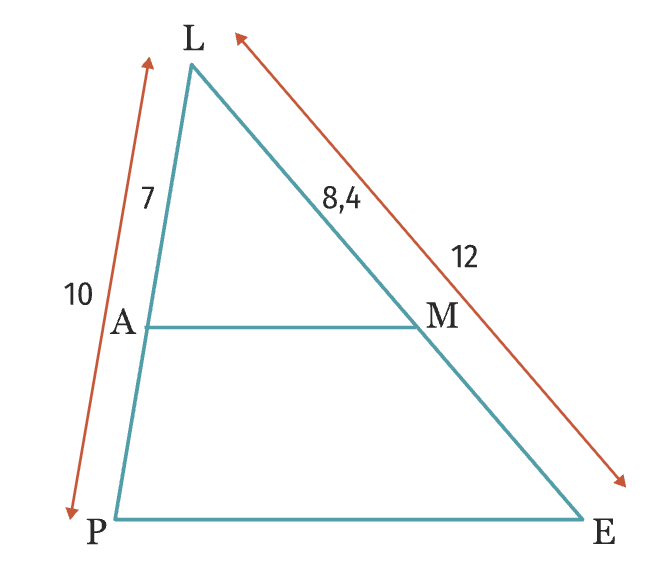
\includegraphics[width=1\textwidth]{fig2.png}
    \end{center}
\end{minipage}%


\vspace{10pt}

\newpage
% ======================================================
\noindent
\textbf{\large{Exercice 3 : Développer et réduire} (\ \ \ \  / 8 points )}

\vspace{5pt}
\begin{questions}
    \question[2] Associer chaque expressions à son expression réduite :

    \begin{center}
        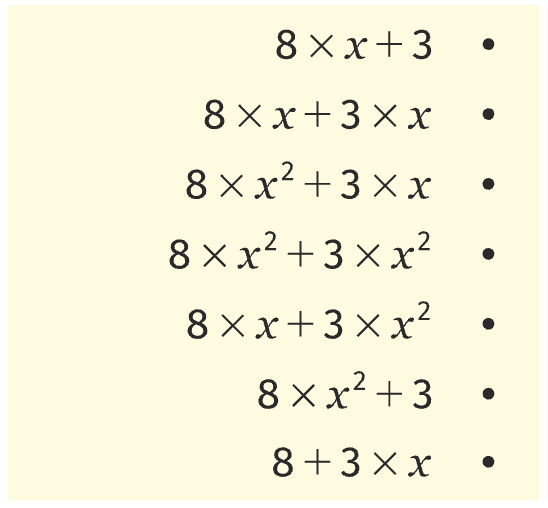
\includegraphics[width=0.27\textwidth]{fig4.png}
        \hspace{2cm}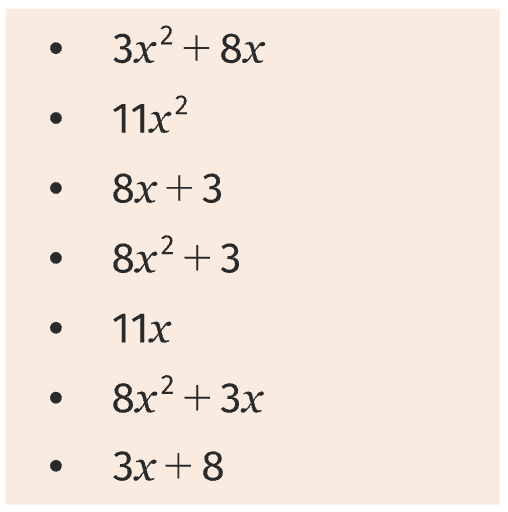
\includegraphics[width=0.25\textwidth]{fig5.png}
    \end{center}

    \question[2] Réduire les expressions suivantes :

    \vspace{5pt}
    \hspace{1cm}a) $6x -4 + 2x + 9 + 5x$

    \vspace{5pt}
    \hspace{1cm}b) $-4x + 6 - 3x^2 + 8x - 4 + 5x^2$

    \vspace{10pt}
    \question[4] Développer les expressions suivantes :
    
    \vspace{5pt}
    \hspace{1cm}a) $-2(x+3)$ \hspace{2cm}b) $-4(x-1)$

    \vspace{5pt}
    \hspace{1cm}c) $7(2x+4)$ \hspace{2.15cm}d) $x(x-5)$
\end{questions}

\vspace{20pt}


\begin{center}
    \textit{Fin du devoir}
\end{center}

\end{document}
